% Source: tex/chapters/ch06/07_ソフトウェアエンジニアリング運用制御.tex
\subsubsection{サービス報告}

サービス報告は、意思決定に必要な、合意済みで、適時で、信頼でき、正確な情報を作る活動である。報告は、運用サービスがどのように機能したか、サービス水準を満たしたか、どの問題が発生したか、今後の傾向がどうかを示す。

典型的な報告項目には、サービス水準目標に対する性能、セキュリティ侵害、トランザクション量、資源使用量、インシデントと失敗、傾向情報、満足度分析がある。測定を自動化し、収集、分析、報告、制御を調整できる枠組みとツールを選定することが重要である。

\begin{figure}[htbp]
\centering
\IfFileExists{assets/generated_figures/ch06/fig-ch06-10.png}{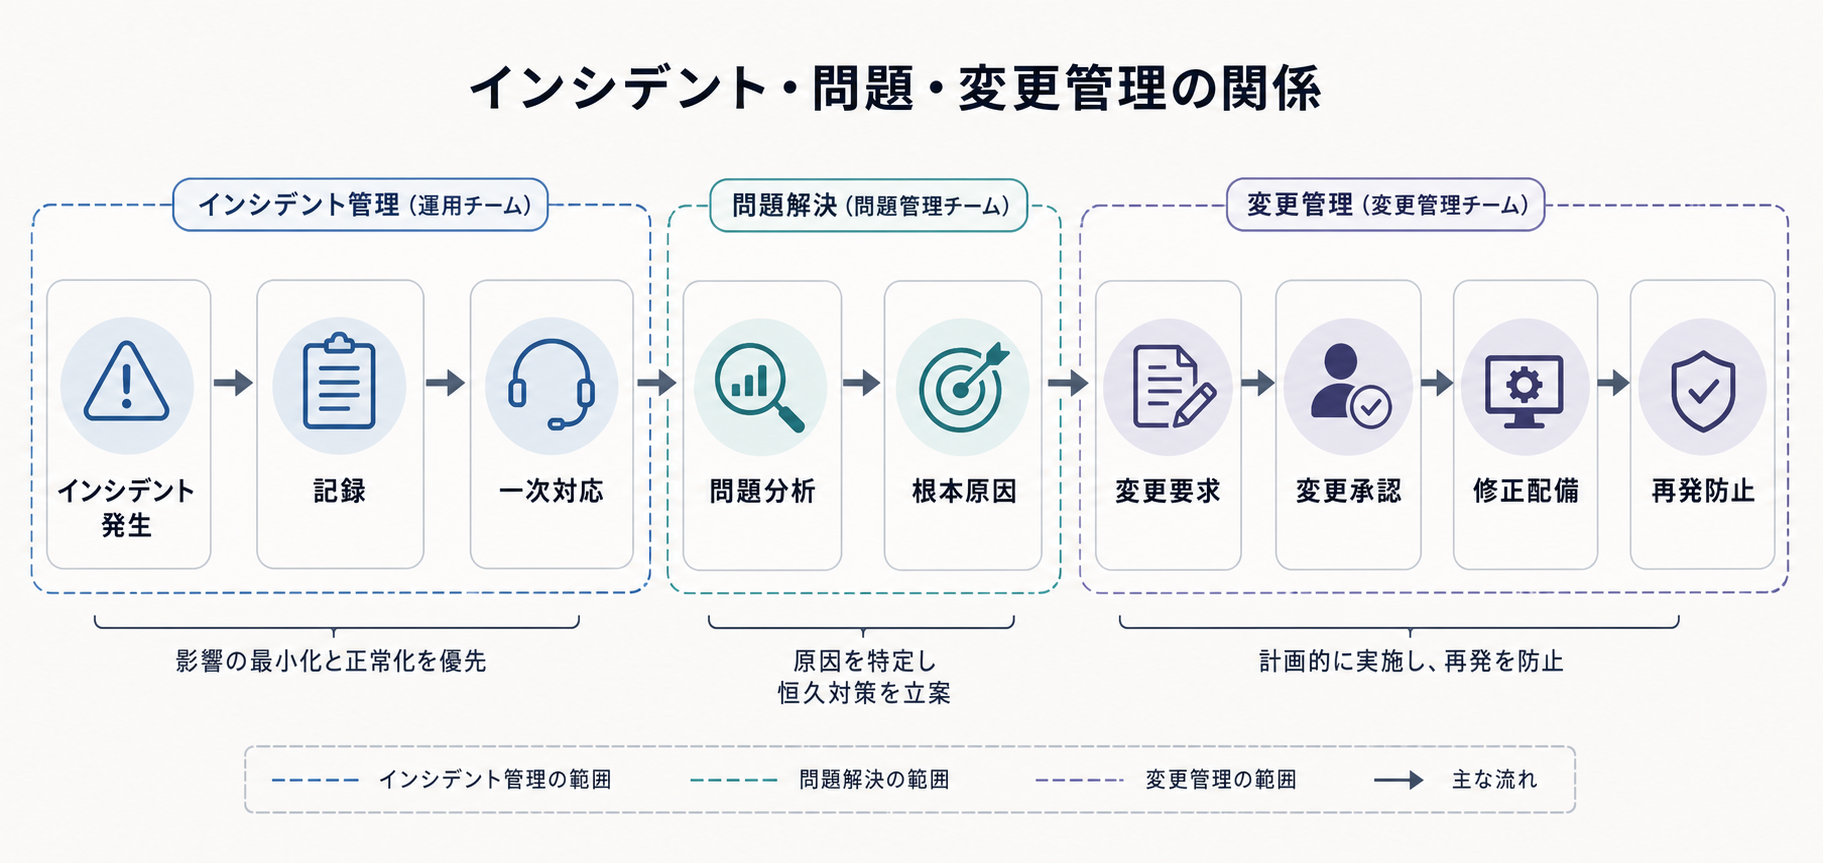
\includegraphics[width=0.96\linewidth]{assets/generated_figures/ch06/fig-ch06-10.png}}{\fbox{\parbox[c][48mm][c]{0.9\linewidth}{\centering 画像生成待ち\\インシデント・問題・変更管理の関係}}}
\caption{インシデント・問題・変更管理の関係}
\label{fig:ch06-10}
\end{figure}
